\usetikzlibrary{calc}
\usetikzlibrary{patterns}
\usetikzlibrary{arrows.meta}

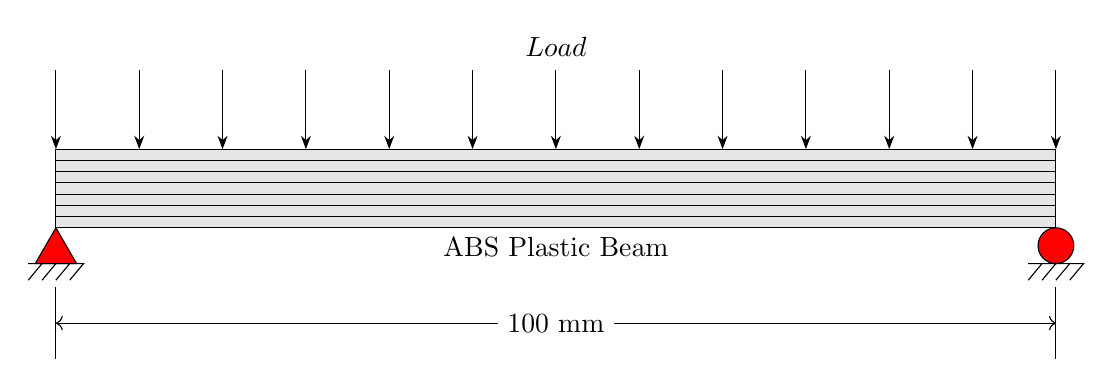
\begin{tikzpicture}


 %% defining the corners of the grill
  \coordinate (grill/sw) at (0,0);
  \coordinate (grill/ne) at ($(grill/sw)+(5in,1cm)$);
  \coordinate (grill/nw) at (grill/sw|-grill/ne);
  \coordinate (grill/se) at (grill/sw-|grill/ne);

  %% filling the grill
  \draw[fill=gray!20] (grill/sw) rectangle (grill/ne);

  %% drawing the horizontal bars of the grill  
  \def\mymax{7}
  \foreach \myn in {0,1,...,\mymax}
  {
    \draw ($(grill/sw)!\myn/\mymax!(grill/nw)$)
       -- ($(grill/se)!\myn/\mymax!(grill/ne)$);
  }

  %% material above the grill 
  %% downward arrows 
  \def\myarrowheight{1cm}
  \def\myarrowcount{12}
  \foreach \myn in {0,1,...,\myarrowcount}
  {
    \draw[arrows=Stealth-] ($(grill/nw)!\myn/\myarrowcount!(grill/ne)$) -- ++ (0,\myarrowheight);
  }
  %% label above downward arrows
  \path ([yshift=\myarrowheight+2ex]grill/nw) --
        ([yshift=\myarrowheight+2ex]grill/ne)
        node[midway] {$Load$};

  %% material below the grill
  %% grill label
  \path (grill/sw) -- (grill/se)  node[midway,below] {ABS Plastic Beam};
  %% corner decorations
  %% isosceles triangle
  \def\myr{1.5ex}
  \draw[fill=red] (grill/sw) -- ++ (-60:{\myr*2/sin(60)})
                             -- ++ (180:{\myr*2/sin(60)})
                             -- cycle;
  %% circle
  \draw[fill=red] ($(grill/se)+(down:\myr)$) circle (\myr);

  %% hash marks under corner decorations
  \begin{scope}[myyshift/.style={yshift={-2*\myr}}]

    \def\mystepmax{4}
    \def\mystepwidth{5pt}
    \def\mystepheight{6pt}
    \foreach \myside in {se,sw}
    {
      \foreach \myn in {1,...,\mystepmax}
      {
        \pgfmathsetmacro\myxshift{ (-\mystepmax /2+\myn)*\mystepwidth  -\mystepwidth}
        \draw ([myyshift,xshift=\myxshift]grill/\myside) --
              ([myyshift,xshift={\myxshift+\mystepwidth}]grill/\myside)   --
              ([myyshift,yshift=-\mystepheight,xshift=\myxshift]grill/\myside);
      } 
    }

  \end{scope}

  \pgfmathsetmacro\myyshift{5ex+2*\myr}
  \begin{scope}[myshift/.style={yshift={-\myyshift}}]

     \path
           ([myshift]grill/sw)
           --
           ([myshift]grill/se)
           node [midway] {100 mm}
           edge[arrows=->] ([myshift]grill/se)
           edge[arrows=->] ([myshift]grill/sw);
     \foreach \myn in {se,sw}
     {
       \draw ([myshift]grill/\myn)
             edge ++(up:3ex)
             edge ++(down:3ex);       
     }  

  \end{scope}

%   \draw ($(grill/ne)+(1cm,0)$) rectangle ($(grill/se)+(1.5cm,0)$);

%   \pattern[pattern=crosshatch dots gray]  ($(grill/ne)+(1cm,0)$) rectangle ($(grill/se)+(1.5cm,0)$);

  
\end{tikzpicture}